%%!TEX TS-program = latex
%\documentclass[10pt,twocolumn,reqno]{amsart}
\documentclass[12pt,reqno]{amsart}
%\usepackage{d:/home/hovey/latexsources/fancyheadings/fancyheadings}
%\usepackage{c:/home/hovey/latexsources/fancyheadings/fancyheadings}
%\usepackage{/Users/Pictor/hovey/latexsources/fancyheadings/fancyheadings} % Pictor
\usepackage{latexsources/fancyheadings/fancyheadings} % Pictor
%\usepackage{d:/home/hovey/latexsources/psfrag}
%\usepackage{c:/home/hovey/latexsources/psfrag}
\usepackage{psfrag}
%\usepackage[foot]{amsaddr}

% two-column: space between columns
\setlength{\columnsep}{1.0cm}

% multi-column spanning
\usepackage{multicol}


\makeatletter
\renewenvironment{quotation}
  {\list{}{\listparindent=1cm
           \itemindent \listparindent
	   \leftmargin=5cm
	   \rightmargin=2cm
	   \topsep=0pt
	   %\parsep \z@ \@plus\p@
	   \sffamily\small}
   \item\relax}
\makeatother

\makeatletter
\newenvironment{question}
  {\list{}{\rule{\textwidth}{0.5pt}
	   \listparindent=0cm
           \itemindent \listparindent
	   \leftmargin=1cm
	   \rightmargin=1cm
	   \topsep=0pt
	   %\parsep \z@ \@plus\p@
	   \sffamily\small\bfseries
	   \rule{3cm}{0.5pt}
	  }
   \item\relax}
\makeatother


\usepackage{color}
\newsavebox{\tempbox}
%
\newcommand{\coloritem}[2]% #1 = color of bar, #2 = item text
{\item \savebox{\tempbox}{\parbox[t]{\linewidth}{#2}}%
  \usebox{\tempbox}\hspace{-\columnwidth}%
    {\color{#1}\rule[-\dp\tempbox]{2pt}{\dimexpr \ht\tempbox+\dp\tempbox}}%
}



%\usepackage{fancyheadings}
%\usepackage[]{psfrag}
%\usepackage{multirow}
\usepackage{epsfig}
\usepackage{pifont} % reqd for dingbats
%\usepackage{subfigure} % requires \usepackage{epsfig} too

%\include{/home/hovey/Hwriting/Hformatams}
%\include{/tmp_mnt/users/lmaf/hovey/Hwriting/Hformatams}
%\include{d:/home/hovey/latexsources/Hformatams}
%\include{c:/home/hovey/latexsources/Hformatams}
%\include{/Users/Pictor/hovey/latexsources/Hformatams} % Pictor
% version 8 Oct 1998 
% Stanford University
% formerly Lausanne, Switzerland


% *-----------------------*
% | LaTeXING THE DOCUMENT |
% *-----------------------*--------------------------------------
%
% Run LaTeX on this file twice for proper section numbers.
% A '%' causes LaTeX to ignore remaining text on the line
% latex filename.tex
% dvips filename.dvi -o filename.ps
% ghostview filename.ps 
%
% *--------------------------------------------------------------


\newcommand{\ie}{{\em i.e., }}
\newcommand{\viz}{{\em viz.}}
\newcommand{\htable}{{\sc Table}}
\newcommand{\hfigure}{{\sc Figure}}

\newcommand{\hframe}[1]{{}^{\mathcal{#1}}\!}

% PLASTICITY - formulation
% ============
 \newcommand{\hstrain}{\varepsilon}
 \newcommand{\vhstrain}{\ve{\varepsilon}}
 \newcommand{\hstraindot}{\dot{\varepsilon}}
 \newcommand{\hstraine}{\varepsilon^{\mbox{\footnotesize e}}}
 \newcommand{\hstrainp}{\varepsilon^{\mbox{\footnotesize p}}}
 \newcommand{\hstrainpdot}{\dot{\varepsilon}^{\mbox{\footnotesize p}}}
 \newcommand{\gammadot}{\dot{\gamma}}
 \newcommand{\sign}{\mbox{sign}}
 \newcommand{\sigmadot}{\dot{\sigma}}  
 \newcommand{\vsigma}{\ve{\sigma}}  
 \newcommand{\Phidot}{\dot{\Phi}}
 \newcommand{\setequal}{\stackrel{\mbox{set}}{=}}
 \newcommand{\Cep}{C_{\mbox{\footnotesize ep}}}
 \newcommand{\Eep}{E_{\mbox{\footnotesize ep}}}
 \newcommand{\keq}{k_{\mbox{\footnotesize eq}}}
 \newcommand{\alphadot}{\dot{\alpha}}

% PLASTICITY - implementation
% ============
 \newcommand{\hstrainn}{\varepsilon_n}
 \newcommand{\hstrainen}{\varepsilon^{\mbox{\footnotesize e}}_{n}}
 \newcommand{\hstrainpn}{\varepsilon^{\mbox{\footnotesize p}}_{n}}
 \newcommand{\alphan}{\alpha_n}
 \newcommand{\gamman}{\gamma_n}
 \newcommand{\hstrainnp}{\varepsilon_{n+1}}
 \newcommand{\hstrainenp}{\varepsilon^{\mbox{\footnotesize e}}_{n+1}}
 \newcommand{\hstrainpnp}{\varepsilon^{\mbox{\footnotesize p}}_{n+1}}
 \newcommand{\hstrainpnpi}{\varepsilon^{\mbox{\footnotesize p}\;(i)}_{n+1}}
 \newcommand{\hstrainpnpip}{\varepsilon^{\mbox{\footnotesize p}\;(i+1)}_{n+1}}
 \newcommand{\hstrainptrnp}{\varepsilon^{\mbox{\footnotesize p tr}}_{n+1}}
 \newcommand{\alphanp}{\alpha_{n+1}}
 \newcommand{\alphanpi}{\alpha_{n+1}^{(i)}}
 \newcommand{\alphatrnp}{\alpha^{\mbox{\footnotesize tr}}_{n+1}}
 \newcommand{\alphanpip}{\alpha_{n+1}^{(i+1)}}
 \newcommand{\gammanp}{\gamma_{n+1}}
 \newcommand{\gammadotnp}{\dot{\gamma}_{n+1}} 

 \newcommand{\sigmatrnp}{\sigma^{\mbox{\footnotesize tr}}_{n+1}}
 \newcommand{\sigman}{\sigma_n}
 \newcommand{\sigmanp}{\sigma_{n+1}}

 \newcommand{\tn}{t_n}
 \newcommand{\tnp}{t_{n+1}}

 \newcommand{\Phinp}{\Phi_{n+1}}
 \newcommand{\Phidotnp}{\dot{\Phi}_{n+1}}
 \newcommand{\Phitrnp}{\Phi^{\mbox{\footnotesize tr}}_{n+1}}

% CIRCLED STATES
% ==============
\newcommand*\circled[1]{\tikz[baseline=(char.base)]{
            \node[shape=circle,draw,inner sep=2pt] (char) {#1};}}

% *--------------*
% | MATH SYMBOLS |
% *--------------*-----------------------------------------------
%
  \newcommand{\hcos}{\sf c}
  \newcommand{\hsin}{\sf s}
  \newcommand{\epi}{\mbox{epi }}
  \newcommand{\fa}{\forall \quad}
  \newcommand{\sotwo}{SO(2)}
  \newcommand{\sothree}{SO(3)}
% \newcommand {\angvel}[3]{{}^{#1}{#2}^{#3}}
% \newcommand{\implies}{\Rightarrow}
  \newcommand{\dirderiv}[1]{\mathbf{D}_{#1}}
  \newcommand{\abs}[1]{| \, #1 \, |}
  \newcommand{\innerproductmap}{\langle \, \cdot \, , \, \cdot \, \rangle}
  \newcommand{\innerproduct}[2]{\langle \, #1    \, , \, #2    \, \rangle}
  \newcommand{\normmap}{\parallel \, \cdot \, \parallel}
  \newcommand{\norm}[1]{\parallel~#1~\parallel}  
  \newcommand{\trace}{\mbox{tr}}
  \newcommand{\DEV}{\mbox{DEV}}
  \newcommand{\dev}{\mbox{dev}}
  \newcommand{\VOL}{\mbox{VOL}}
  \newcommand{\vol}{\mbox{vol}}
  \newcommand{\smDEV}{\mbox{\tiny DEV}}
  \newcommand{\smdev}{\mbox{\tiny dev}}
  \newcommand{\smVOL}{\mbox{\tiny VOL}}
  \newcommand{\smvol}{\mbox{\tiny vol}}
  \newcommand{\DEVoper}{\mbox{DEV}[\;\cdot\;]}
  \newcommand{\devoper}{\mbox{dev}[\;\cdot\;]}
  \newcommand{\ltwonorm}[1]{\parallel #1 \parallel_{_2}}
  \newcommand{\st}{\mbox{s.t. }}
  \newcommand{\pd}{\mbox{p.d. }}
  \newcommand{\defe}{\stackrel{\Delta}{=}}
  \newcommand{\dst}{\displaystyle} 
  \newcommand{\be}{\begin{equation}}
  \newcommand{\ee}{\end{equation}}
% \newcommand{\ve}[1]{\mathbf{#1}}
  \newcommand{\ve}[1]{\mbox{\boldmath $#1$}}
  \newcommand{\half}{\frac{1}{2}}


% the old diad that I commented out 5/24/96
% \newcommand{\di}[1]{\mathsf{#1}}
% this new one seems to work, helvetica under the file
% /usr/local/teTeX/texmf/fonts/tfm/adobe/helvetic/phvb8r.tfm
%  \font\gm=msym10  % <- this one doesn't work
  \font\gm=phvb8r   % this is helvetica font essentially
  \newcommand{\di}[1]{\hbox{\gm #1}}
  \font\idm=zptmcmrm
  \newcommand{\dii}{\hbox{\idm I}}
  \font\zaph=pzcmi8t
  \newcommand{\refframe}[1]{\hbox{\zaph #1}}

% \newcommand{\di}[1]{\hbox{\tenbfss #1}}
  \newcommand{\dib}[1]{\bf \mathsf{#1} }
%  \newcommand{\qed}{{\;\; \blacksquare} }
%
% *--------------------------------------------------------------

% BIOMECHANICS
% ============
\newcommand{\Pmtar}{P_{\mbox{\tiny mtar}}}
\newcommand{\Pheel}{P_{\mbox{\tiny heel}}}

 
% VECTOR CALCULUS OPERATORS
% =========================

\newcommand{\gradX}{\ve{\nabla}}
\newcommand{\gradx}{\ve{\nabla}_{x}}
\renewcommand{\div}{\cdot}
\newcommand{\vdiv}{\ve{\cdot}}
\newcommand{\ddiv}{:}
\newcommand{\vddiv}{\ve{:}}
\newcommand{\union}{\cup}
\newcommand{\intersection}{\cap}

\newcommand{\DIV}{\mbox{DIV}}
%\newcommand{\div}{\mbox{div}}


% DINGBATS (CIRLED NUMBERS)
% (MUST ALSO HAVE \usepackage{pifont} IN HEADER
% =============================================
\newcommand{\circleone}{{\mbox{\small \ding{172}}}}
\newcommand{\circletwo}{{\mbox{\small \ding{173}}}}

% VECTOR ALPHABET
% ===============

\newcommand{\vA}{\ve{A}}
\newcommand{\va}{\ve{a}}
\newcommand{\Dva}{\Delta \va}
\newcommand{\vB}{\ve{B}}
\newcommand{\vb}{\ve{b}}
\newcommand{\vC}{\ve{C}}
\newcommand{\vCdot}{\dot{\ve{C}}}
\newcommand{\vCinv}{\ve{C}^{-1}}
\newcommand{\vc}{\ve{c}}
\newcommand{\vD}{\ve{D}}
\newcommand{\vd}{\ve{d}}
\newcommand{\Dvd}{\Delta \vd}
\newcommand{\vE}{\ve{E}}
\newcommand{\vEdot}{\dot{\ve{E}}}
\newcommand{\vF}{\ve{F}}
\newcommand{\vFdot}{\dot{\ve{F}}}
\newcommand{\vf}{\ve{f}}
\newcommand{\vG}{\ve{G}}
\newcommand{\vg}{\ve{g}}
\newcommand{\gdot}{\dot{g}}
\newcommand{\vH}{\ve{H}}
\newcommand{\vh}{\ve{h}}
\newcommand{\vI}{\ve{I}}
\newcommand{\vid}{\ve{1}}
\newcommand{\vJ}{\ve{J}}
\newcommand{\vK}{\ve{K}}
%\newcommand{\vKe}{\ve{K}^{\mbox{\tiny e}}} % already defined
\newcommand{\vL}{\ve{L}}
\newcommand{\vl}{\ve{l}}
\newcommand{\vM}{\ve{M}}
\newcommand{\vN}{\ve{N}}
\newcommand{\vn}{\ve{n}}
\newcommand{\vO}{\ve{O}}
\newcommand{\vP}{\ve{P}}
\newcommand{\vp}{\ve{p}}
\newcommand{\vPelas}{\ve{P}^{\mbox{\tiny elas}}}
\newcommand{\vPvisc}{\ve{P}^{\mbox{\tiny visc}}}
\newcommand{\vQ}{\ve{Q}}
\newcommand{\vq}{\ve{q}}
\newcommand{\vqdot}{\dot{\ve{q}}}
\newcommand{\vqddot}{\ddot{\ve{q}}}
\newcommand{\vR}{\ve{R}}
\newcommand{\vr}{\ve{r}}
\newcommand{\vrhat}{\hat{\ve{r}}}
\newcommand{\vS}{\ve{S}}
\newcommand{\vSelas}{\ve{S}^{\mbox{\tiny elas}}} 
\newcommand{\vSvisc}{\ve{S}^{\mbox{\tiny visc}}}
\newcommand{\vs}{\ve{s}}
\newcommand{\vsdot}{\dot{\ve{s}}}
\newcommand{\vsddot}{\ddot{\ve{s}}}
\newcommand{\vshat}{\hat{\ve{s}}}
\newcommand{\vT}{\ve{T}}
\newcommand{\vTbar}{\bar{\ve{T}}}
\newcommand{\vThat}{\hat{\ve{T}}}
\newcommand{\vTT}{\vT_{\mbox{\tiny T}}}
\newcommand{\vt}{\ve{t}}
\newcommand{\vthat}{\hat{\ve{t}}}
\newcommand{\vU}{\ve{U}}
\newcommand{\vUbar}{\bar{\ve{U}}}
\newcommand{\vUdot}{\dot{\ve{U}}}
\newcommand{\vUddot}{\ddot{\ve{U}}}
\newcommand{\vu}{\ve{u}}
\newcommand{\DvU}{\Delta \vU}
\newcommand{\vV}{\ve{V}}
\newcommand{\vv}{\ve{v}}
\newcommand{\Dvv}{\Delta \vv}
\newcommand{\vW}{\ve{W}}
\newcommand{\vw}{\ve{w}}
\newcommand{\vX}{\ve{X}}
\newcommand{\vx}{\ve{x}}
\newcommand{\vxhat}{\hat{\ve{x}}}
\newcommand{\vY}{\ve{Y}}
\newcommand{\vy}{\ve{y}}
\newcommand{\vyhat}{\hat{\ve{y}}}
\newcommand{\vZ}{\ve{Z}}
\newcommand{\vz}{\ve{z}}

% VECTOR NUMBERS
% ==============
  \newcommand{\vzero}{\ve{0}}

% BLACKBOARD ALPHABET
% ===================
  \newcommand{\dist}{\mathbb{D}}
  \newcommand{\proj}{\mathbb{P}}
  \newcommand{\projT}{\proj_{\mbox{\tiny T}}}
  \newcommand{\interval}{\mathbb{T}}

% VECTOR GREEK ALPHABET
% =====================
  \newcommand{\vDelta}{\ve{\Delta}}
  \newcommand{\vdelta}{\ve{\delta}}
  \newcommand{\vkappa}{\ve{\kappa}}
  \newcommand{\vLambda}{\ve{\Lambda}}
  \newcommand{\vlambda}{\ve{\lambda}}
  \newcommand{\vphi}{\ve{\phi}}
  \newcommand{\vvarphi}{\ve{\varphi}}
  \newcommand{\vvarphidot}{\dot{\ve{\varphi}}}
  \newcommand{\vvarphiddot}{\ddot{\ve{\varphi}}}
  \newcommand{\vxi}{\ve{\xi}}
  \newcommand{\vthetahat}{\hat{\ve{\theta}}}
  \newcommand{\vtau}{\ve{\tau}}

% CALIGRAPHY ALPHABET
% ===================
  \newcommand{\cA}{\mathcal{A}}
  \newcommand{\cB}{\mathcal{B}}
  \newcommand{\cC}{\mathcal{C}}
  \newcommand{\cD}{\mathcal{D}}
  \newcommand{\cE}{\mathcal{E}}
  \newcommand{\cF}{\mathcal{F}}
  \newcommand{\cG}{\mathcal{G}}
  \newcommand{\cI}{\mathcal{I}}
  \newcommand{\cJ}{\mathcal{J}}
  \newcommand{\cK}{\mathcal{K}}
  \newcommand{\cL}{\mathcal{L}}
  \newcommand{\cO}{\mathcal{O}}
  \newcommand{\cP}{\mathcal{P}}
  \newcommand{\cQ}{\mathcal{Q}}
  \newcommand{\cR}{\mathcal{R}}  
  \newcommand{\cS}{\mathcal{S}}
  \newcommand{\cV}{\mathcal{V}}
  \newcommand{\cW}{\mathcal{W}}


% ENERGY ALPHABET
% ===============
  \newcommand{\Vext}{V^{\mbox{\tiny ext}}}
  \newcommand{\Vint}{V^{\mbox{\tiny int}}}

% Fourth Order Tensor ALPHABET
% ============================
%\newcommand{\tC}{\mathbb{C}}
%\newcommand{\tI}{\mathbb{I}}
%\newcommand{\tV}{\mathbb{V}}

\newcommand{\tA}{\mbox{\sffamily A}}
\newcommand{\tC}{\mbox{\sffamily C}}
\newcommand{\tI}{\mbox{\rmfamily I}}
\newcommand{\tV}{\mbox{\sffamily V}}

\newcommand{\tCbold}{\mbox{\sffamily\bfseries C}}
\newcommand{\tIbold}{\mbox{\rmfamily\bfseries I}}
\newcommand{\tVbold}{\mbox{\sffamily\bfseries V}}

\newcommand{\tICinv}{\tIbold_{C^{-1}}}

\newcommand{\tc}{\mbox{\sffamily\large c}}
\newcommand{\ti}{\mbox{\rmfamily\large i}}
\newcommand{\tv}{\mbox{\sffamily\large v}}

\newcommand{\tcbold}{\mbox{\sffamily\bfseries\large c}}
\newcommand{\tibold}{\mbox{\rmfamily\bfseries\large i}}
\newcommand{\tvbold}{\mbox{\sffamily\bfseries\large v}}

%\newcommand{\assembly}{\overset{n_{el}}{\underset{e=1}{
%  \mbox{ \sffamily\bfseries \large A } }}}

% Tensor INVARIANTS
% =================
\newcommand{\invCone}{\mbox{\rmfamily I}_C}
\newcommand{\invCtwo}{\mbox{\rmfamily II}_C}
\newcommand{\invCthree}{\mbox{\rmfamily III}_C}

% RIGID BODY  NOTATION
% ====================
% plain variable
\newcommand{\vucm}{\overset{*}{\ve{u}}}
\newcommand{\vvcm}{\overset{*}{\ve{v}}}
\newcommand{\vacm}{\overset{*}{\ve{a}}}
\newcommand{\vXcm}{\overset{*}{\ve{X}}}
\newcommand{\Xcm}{\overset{*}{X}}
\newcommand{\vxcm}{\overset{*}{\ve{x}}}
\newcommand{\vvarphicm}{\overset{*}{\ve{\varphi}}}
\newcommand{\vtheta}{\ve{\theta}}
\newcommand{\thetadot}{\dot{\theta}}
\newcommand{\vthetadot}{\dot{\ve{\theta}}}
\newcommand{\vthetaddot}{\ddot{\ve{\theta}}}
\newcommand{\vomega}{\ve{\omega}}
\newcommand{\vpsi}{\ve{\psi}}
\newcommand{\psidot}{\dot{\psi}}
\newcommand{\vpsidot}{\dot{\ve{\psi}}}
\newcommand{\valpha}{\ve{\alpha}}
\newcommand{\vpi}{\ve{\pi}}

\newcommand{\vvCinB}{}

%  at time n
\newcommand{\vucmn}{\overset{*}{\ve{u}}_n}
\newcommand{\vvcmn}{\overset{*}{\ve{v}}_n}
\newcommand{\vacmn}{\overset{*}{\ve{a}}_n}
\newcommand{\vXcmn}{\overset{*}{\ve{X}}_n}
\newcommand{\vxcmn}{\overset{*}{\ve{x}}_n}
\newcommand{\vvarphicmn}{\overset{*}{\ve{\varphi}}_n}
\newcommand{\vthetan}{\ve{\theta}_n}
\newcommand{\vthetadotn}{\dot{\ve{\theta}}_n}
\newcommand{\vthetaddotn}{\ddot{\ve{\theta}}_n}
\newcommand{\vomegan}{\ve{\omega}_n}
\newcommand{\valphan}{\ve{\alpha}_n}

% at time n+1
\newcommand{\vucmnp}{\overset{*}{\ve{u}}_{n+1}}
\newcommand{\vvcmnp}{\overset{*}{\ve{v}}_{n+1}}
\newcommand{\vacmnp}{\overset{*}{\ve{a}}_{n+1}}
\newcommand{\vXcmnp}{\overset{*}{\ve{X}}_{n+1}}
\newcommand{\vxcmnp}{\overset{*}{\ve{x}}_{n+1}}
\newcommand{\vvarphicmnp}{\overset{*}{\ve{\varphi}}_{n+1}}
\newcommand{\vthetanp}{\ve{\theta}_{n+1}}
\newcommand{\vthetadotnp}{\dot{\ve{\theta}}_{n+1}}
\newcommand{\vthetaddotnp}{\ddot{\ve{\theta}}_{n+1}}
\newcommand{\vomeganp}{\ve{\omega}_{n+1}}
\newcommand{\valphanp}{\ve{\alpha}_{n+1}}

% at time n+1 iteration i
\newcommand{\vucmnpi}{\overset{*}{\ve{u}}_{n+1}^{(i)}}
\newcommand{\vvcmnpi}{\overset{*}{\ve{v}}_{n+1}^{(i)}}
\newcommand{\vacmnpi}{\overset{*}{\ve{a}}_{n+1}^{(i)}}
\newcommand{\vXcmnpi}{\overset{*}{\ve{X}}_{n+1}^{(i)}}
\newcommand{\vxcmnpi}{\overset{*}{\ve{x}}_{n+1}^{(i)}}
\newcommand{\vvarphicmnpi}{\overset{*}{\ve{\varphi}}_{n+1}^{(i)}}
\newcommand{\Dvucmnpi}{\Delta \overset{*}{\ve{u}}_{n+1}^{(i)}}
\newcommand{\vthetanpi}{\ve{\theta}_{n+1}^{(i)}}
\newcommand{\vthetadotnpi}{\dot{\ve{\theta}}_{n+1}^{(i)}}
\newcommand{\vthetaddotnpi}{\ddot{\ve{\theta}}_{n+1}^{(i)}}
\newcommand{\vomeganpi}{\ve{\omega}_{n+1}^{(i)}}
\newcommand{\valphanpi}{\ve{\alpha}_{n+1}^{(i)}}


% at time n+1 iteration i+1
\newcommand{\vucmnpip}{\overset{*}{\ve{u}}_{n+1}^{(i+1)}}
\newcommand{\vvcmnpip}{\overset{*}{\ve{v}}_{n+1}^{(i+1)}}
\newcommand{\vacmnpip}{\overset{*}{\ve{a}}_{n+1}^{(i+1)}}
\newcommand{\vXcmnpip}{\overset{*}{\ve{X}}_{n+1}^{(i+1)}}
\newcommand{\vxcmnpip}{\overset{*}{\ve{x}}_{n+1}^{(i+1)}}
\newcommand{\vvarphicmnpip}{\overset{*}{\ve{\varphi}}_{n+1}^{(i+1)}}
\newcommand{\vthetanpip}{\ve{\theta}_{n+1}^{(i+1)}}
\newcommand{\vthetadotnpip}{\dot{\ve{\theta}}_{n+1}^{(i+1)}}
\newcommand{\vthetaddotnpip}{\ddot{\ve{\theta}}_{n+1}^{(i+1)}}
\newcommand{\vomeganpip}{\ve{\omega}_{n+1}^{(i+1)}}
\newcommand{\valphanpip}{\ve{\alpha}_{n+1}^{(i+1)}}


% volumes and other geometry
\newcommand{\OmegaR}{\Omega_R}
\newcommand{\intOmegaR}{\int_{\Omega_R}}
\newcommand{\intOmegaRe}{\int_{\Omega_R^e}}
\newcommand{\OmegaOne}{\Omega_1}
\newcommand{\OmegaTwo}{\Omega_2}

% masses and ineritas
%\newcommand{\inertia}{{\mbox{\rmfamily\bfseries I}}}
%\newcommand{\inertiaJ}{{\mbox{\rmfamily\bfseries J}}}
\newcommand{\inertia}{\mathbb I}
\newcommand{\inertiaJ}{\mathbb J}

% inertia at time n
\newcommand{\inertian}{{\mathbb I}_n}
\newcommand{\inertiaJn}{{\mathbb J}_n}

% END RIGID BODY NOTATION
% =======================


% *---------------*
% | BASIS VECTORS |
% *---------------*----------------------------------------------

%\newcommand{\veaa}{\hat{\ve{e}}_{01}}
%\newcommand{\veab}{\hat{\ve{e}}_{02}}
%\newcommand{\veac}{\hat{\ve{e}}_{03}}
%\newcommand{\veaa}{^{A}\hat{\ve{e}}_{1}}
%\newcommand{\veab}{^{A}\hat{\ve{e}}_{2}}
%\newcommand{\veac}{^{A}\hat{\ve{e}}_{3}}
%\newcommand{\veaa}{\hat{\ve{a}}_{1}}
%\newcommand{\veab}{\hat{\ve{a}}_{2}}
%\newcommand{\veac}{\hat{\ve{a}}_{3}}
\newcommand{\vea}{\hat{\ve{\sf{a}}}}
\newcommand{\veaa}{\hat{\ve{\sf{a}}}_1}
\newcommand{\veab}{\hat{\ve{\sf{a}}}_2}
\newcommand{\veac}{\hat{\ve{\sf{a}}}_3}
%
%\newcommand{\veba}{\hat{\ve{e}}_{11}}
%\newcommand{\vebb}{\hat{\ve{e}}_{12}}
%\newcommand{\vebc}{\hat{\ve{e}}_{13}}
%\newcommand{\veba}{\hat{\ve{b}}_{1}}
%\newcommand{\vebb}{\hat{\ve{b}}_{2}}
%\newcommand{\vebc}{\hat{\ve{b}}_{3}}
\newcommand{\veb}{\hat{\ve{\sf{b}}}}
\newcommand{\veba}{\hat{\ve{\sf{b}}}_1}
\newcommand{\vebb}{\hat{\ve{\sf{b}}}_2}
\newcommand{\vebc}{\hat{\ve{\sf{b}}}_3}
%

%\newcommand{\veca}{\hat{\ve{e}}_{21}}
%\newcommand{\vecb}{\hat{\ve{e}}_{22}}
%\newcommand{\vecc}{\hat{\ve{e}}_{23}}
\newcommand{\veca}{\hat{\ve{c}}_{1}}
\newcommand{\vecb}{\hat{\ve{c}}_{2}}
\newcommand{\vecc}{\hat{\ve{c}}_{3}}
%%
\newcommand{\veda}{\hat{\ve{e}}_{31}}
\newcommand{\vedb}{\hat{\ve{e}}_{32}}
\newcommand{\vedc}{\hat{\ve{e}}_{33}}
%
\newcommand{\veea}{\hat{\ve{e}}_{41}}
\newcommand{\veeb}{\hat{\ve{e}}_{42}}
\newcommand{\veec}{\hat{\ve{e}}_{43}}
%
%\newcommand{\veca}{\hat{\ve{e}}_{\cC1}}
%\newcommand{\vecb}{\hat{\ve{e}}_{\cC2}}
%\newcommand{\vecc}{\hat{\ve{e}}_{\cC3}}
%
%\newcommand{\vefa}{\hat{\ve{e}}_{\cF1}}
%\newcommand{\vefb}{\hat{\ve{e}}_{\cF2}}
%\newcommand{\vefc}{\hat{\ve{e}}_{\cF3}}
\newcommand{\vefa}{\hat{\ve{\sf{f}}}_1}
\newcommand{\vefb}{\hat{\ve{\sf{f}}}_2}
\newcommand{\vefc}{\hat{\ve{\sf{f}}}_3}



%
\newcommand{\veva}{\hat{\ve{e}}_{\cV1}}
\newcommand{\vevb}{\hat{\ve{e}}_{\cV2}}
\newcommand{\vevc}{\hat{\ve{e}}_{\cV3}}


\newcommand{\veihat}{\hat{\ve{\sf{i}}}}
\newcommand{\vejhat}{\hat{\ve{\sf{j}}}}
\newcommand{\vekhat}{\hat{\ve{\sf{k}}}}


% FEA OPERATOR NOTATION
% =====================
\newcommand{\Moper}{\mathcal{M}(\cdot,\cdot)}
\newcommand{\Meoper}{\mathcal{M}(\cdot,\cdot)^e}
\newcommand{\Noper}{\mathcal{N}(\cdot;\cdot,\cdot)}
\newcommand{\Neoper}{\mathcal{N}(\cdot;\cdot,\cdot)^e}
\newcommand{\Boper}{(\cdot,\cdot)}
\newcommand{\Beoper}{(\cdot,\cdot)^e}
\newcommand{\Toper}{(\cdot,\cdot)_{\Gamma_H}}
\newcommand{\Teoper}{(\cdot,\cdot)^e_{\Gamma_H}}

% FEA INTEGERS
% ============
\newcommand{\nel}{n_{\mbox{\tiny el}}}
\newcommand{\nen}{n_{\mbox{\tiny en}}}
\newcommand{\nsd}{n_{\mbox{\tiny sd}}}
%\newcommand{\neq}{n_{\mbox{\tiny eq}}}
\newcommand{\numeq}{n_{\mbox{\tiny eq}}}
\newcommand{\nts}{n_{\mbox{\tiny ts}}}
\newcommand{\naf}{n_{\mbox{\tiny af}}}
\newcommand{\nam}{n_{\mbox{\tiny am}}}
\newcommand{\nat}{n_{\mbox{\tiny at}}}

\newcommand{\GDYN}{G_{\mbox{\tiny DYN}}}

% SHAPE FUNCTION TRIAL FUNCTION
% =============================

\newcommand{\Uh}{U^h}
\newcommand{\Uhi}{U^h_i}
\newcommand{\vUh}{\ve{U}^h}
\newcommand{\vUt}{\ve{U}_t}
\newcommand{\vUhdot}{\dot{\ve{U}}^h}

\newcommand{\Wh}{W^h}
\newcommand{\Whi}{W^h_i}
\newcommand{\vWh}{\ve{W}^h}

\newcommand{\vTt}{\ve{T}_t}

\newcommand{\Kh}{K^h}
\newcommand{\Khi}{K^h_i}
\newcommand{\vKh}{\ve{K}^h}

\newcommand{\vcK}{\ve{\mathcal{K}}}
\newcommand{\vcKh}{\ve{\mathcal{K}}^h}
\newcommand{\vcV}{\ve{\mathcal{V}}}
\newcommand{\vcVh}{\ve{\mathcal{V}}^h}
\newcommand{\vcW}{\ve{\mathcal{W}}}
\newcommand{\vcWh}{\ve{\mathcal{W}}^h}
\newcommand{\vcS}{\ve{\mathcal{S}}}
\newcommand{\vcSh}{\ve{\mathcal{S}}^h}
\newcommand{\vcC}{\ve{\mathcal{C}}}

% RIGID BODY MASS CENTERS
% =======================
\newcommand{\Bstar}{B^{*}}

% INTEGRATION SYMBOLS
% ===================

\newcommand{\Omegae}{\Omega^e}

\newcommand{\intBox}{\int_{\Box}}

\newcommand{\intOmega}{\int_{\Omega}}
\newcommand{\intOmegae}{\int_{\Omega^e}}
\newcommand{\intomega}{\int_{\omega}}
\newcommand{\intomegae}{\int_{\omega^e}}


\newcommand{\intGamma}{\int_{\Gamma}}
\newcommand{\intgamma}{\int_{\gamma}}
\newcommand{\intGammaH}{\int_{\Gamma_H}}
\newcommand{\intGammaT}{\int_{\Gamma_T}}
\newcommand{\intGammaU}{\int_{\Gamma_U}}
\newcommand{\intGammaC}{\int_{\Gamma_C}}
\newcommand{\intGammaHe}{\int_{\Gamma^e_H}}
\newcommand{\intgammah}{\int_{\gamma_h}}

\newcommand{\intOmegaalpha}{\int_{\Omega^{(\alpha)}}}
\newcommand{\intGammaalpha}{\int_{\Gamma^{(\alpha)}}}
\newcommand{\intGammaone}{\int_{\Gamma^{(1)}}}
\newcommand{\intGammatwo}{\int_{\Gamma^{(2)}}}
\newcommand{\intGammaTalpha}{\int_{\Gamma_T^{(\alpha)}}}
\newcommand{\intGammaCalpha}{\int_{\Gamma_C^{(\alpha)}}}
\newcommand{\intGammaCone}{\int_{\Gamma_C^{(1)}}}
\newcommand{\intGammaCtwo}{\int_{\Gamma_C^{(2)}}}

\newcommand{\GammaH}{\Gamma_{H}}


\newcommand{\dOmega}{\; d\Omega}
\newcommand{\domega}{\; d\omega}
\newcommand{\dGamma}{\; d\Gamma}
\newcommand{\dgamma}{\; d\gamma}
\newcommand{\dGammaC}{\; d\Gamma_C}
\newcommand{\dBox}{\; d\;\Box}
\newcommand{\dOmegaalpha}{\; d\Omega^{(\alpha)}} 
\newcommand{\dGammaalpha}{\; d\Gamma^{(\alpha)}}

\newcommand{\deltae}{\delta^{\mbox{\tiny e}}}
\newcommand{\vdeltae}{\ve{\delta}^{\mbox{\tiny e}}}
\newcommand{\Deltae}{\Delta^{\mbox{\tiny e}}}
\newcommand{\vDeltae}{\ve{\Delta}^{\mbox{\tiny e}}}
 
\newcommand{\sone}{^{(1)}}
\newcommand{\stwo}{^{(2)}}
\newcommand{\sa}{^{(\alpha)}}


% *-----------------------------*
% | STRUCTURAL DYNAMICS SYMBOLS |
% *-----------------------------*--------------------------------

%\newcommand{\vd}{\ve{d}}
%\newcommand{\vv}{\ve{v}}
%\newcommand{\va}{\ve{a}}

\newcommand{\vdn}{\ve{d}_{n}}
\newcommand{\vun}{\ve{u}_{n}}
\newcommand{\vue}{\ve{u}^{\mbox{\tiny e}}}
\newcommand{\vUn}{\ve{U}_{n}}
\newcommand{\vvn}{\ve{v}_{n}}
\newcommand{\van}{\ve{a}_{n}}

\newcommand{\vdnp}{\ve{d}_{n+1}}
\newcommand{\vunp}{\ve{u}_{n+1}}
\newcommand{\vUnp}{\ve{U}_{n+1}}
\newcommand{\vvnp}{\ve{v}_{n+1}}
\newcommand{\vanp}{\ve{a}_{n+1}}

\newcommand{\vdnpa}{\ve{d}_{n+\alpha}}
\newcommand{\vunpa}{\ve{u}_{n+\alpha}}
\newcommand{\vUnpa}{\ve{U}_{n+\alpha}}
\newcommand{\vvnpa}{\ve{v}_{n+\alpha}}
\newcommand{\vVnpa}{\ve{V}_{n+\alpha}}
\newcommand{\vanpa}{\ve{a}_{n+\alpha}}
\newcommand{\vAnpa}{\ve{A}_{n+\alpha}}


\newcommand{\vdnm}{\ve{d}_{n-1}}
\newcommand{\vunm}{\ve{u}_{n-1}}
\newcommand{\vvnm}{\ve{v}_{n-1}}
\newcommand{\vanm}{\ve{a}_{n-1}}

\newcommand{\vdni}{\ve{d}_{n}^{(i)}}
\newcommand{\vuni}{\ve{u}_{n}^{(i)}}
\newcommand{\vUni}{\ve{U}_{n}^{(i)}}
\newcommand{\vvni}{\ve{v}_{n}^{(i)}}
\newcommand{\vani}{\ve{a}_{n}^{(i)}}

\newcommand{\vdnpi}{\ve{d}_{n+1}^{(i)}}
\newcommand{\vunpi}{\ve{u}_{n+1}^{(i)}}
\newcommand{\vUnpi}{\ve{U}_{n+1}^{(i)}}
\newcommand{\vvnpi}{\ve{v}_{n+1}^{(i)}}
\newcommand{\vanpi}{\ve{a}_{n+1}^{(i)}}

\newcommand{\vdnpip}{\ve{d}_{n+1}^{(i+1)}}
\newcommand{\vunpip}{\ve{u}_{n+1}^{(i+1)}}
\newcommand{\vVnpip}{\ve{U}_{n+1}^{(i+1)}}
\newcommand{\vvnpip}{\ve{v}_{n+1}^{(i+1)}}
\newcommand{\vanpip}{\ve{a}_{n+1}^{(i+1)}}

%\newcommand{\vM}{\ve{M}}
\newcommand{\vMs}{\ve{M}^{*}}
\newcommand{\vMnpi}{\vM_{n+1}^{(i)}}
%\newcommand{\vC}{\ve{C}}
\newcommand{\vDnpi}{\vD_{n+1}^{(i)}}
%\newcommand{\vK}{\ve{K}}
\newcommand{\vKe}{\ve{K}^{\mbox{\tiny e}}}
\newcommand{\vKd}{\ve{K}(\ve{d})}
\newcommand{\vKnpi}{\ve{K}_{n+1}^{(i)}}
%\newcommand{\vN}{\ve{N}}
\newcommand{\vNd}{\ve{N}(\ve{d})}
\newcommand{\vNdn}{\ve{N}(\ve{d}_{n})}
\newcommand{\vNdnp}{\ve{N}(\ve{d}_{n+1})}
\newcommand{\vNdnpi}{\ve{N}(\ve{d}_{n+1}^{(i)})}
\newcommand{\vNdnpip}{\ve{N}(\ve{d}_{n+1}^{(i+1)})}

\newcommand{\vVn}{\ve{V}_{n}}
\newcommand{\vVnp}{\ve{V}_{n+1}}

\newcommand{\vvarphin}{\ve{\varphi}_{n}}
\newcommand{\vvarphinp}{\ve{\varphi}_{n+1}}
\newcommand{\vvarphinpa}{\ve{\varphi}_{n+\alpha}}


\newcommand{\vFint}{\ve{F}^{\mbox{\tiny int}}}
\newcommand{\vFinte}{\ve{F}^{\mbox{\tiny int,e}}}
\newcommand{\vFintvisc}{\ve{F}^{\mbox{\tiny int,visc}}}
\newcommand{\vFintelas}{\ve{F}^{\mbox{\tiny int,elas}}}
\newcommand{\vFiner}{\ve{F}^{\mbox{\tiny iner}}}
\newcommand{\vFext}{\ve{F}^{\mbox{\tiny ext}}}
\newcommand{\vFexte}{\ve{F}^{\mbox{\tiny ext,e}}}
\newcommand{\vFextn}{\vFext(t_{n})}
\newcommand{\vFextnp}{\vFext(t_{n+1})}
\newcommand{\vFextnpa}{\vFext(t_{n+1+\alpha})}
\newcommand{\vFapp}{\ve{F}^{\mbox{\tiny app}}}

\newcommand{\vMext}{\ve{M}^{ext}}
\newcommand{\vMapp}{\ve{M}^{\mbox{\tiny app}}}
\newcommand{\vTapp}{\ve{T}^{\mbox{\tiny app}}}



\newcommand{\vfint}{\ve{f}^{\mbox{\tiny int}}}
\newcommand{\vfext}{\ve{f}^{\mbox{\tiny ext}}}
\newcommand{\vfextn}{\vfext(t_{n})}
\newcommand{\vfextnp}{\vfext(t_{n+1})}
\newcommand{\vfextnpa}{\vfext(t_{n+1+\alpha})}

\newcommand{\vddd}{\ddot{\ve{d}}}
\newcommand{\vdd}{\dot{\ve{d}}}
% \newcommand{\vd}{\ve{d}}  % already defined above


\newcommand{\pvd}{\tilde{\ve{d}}}
\newcommand{\pvu}{\tilde{\ve{u}}}
\newcommand{\pvv}{\tilde{\ve{v}}}
\newcommand{\pva}{\tilde{\ve{a}}}
\newcommand{\pvvarphi}{\tilde{\ve{\varphi}}}

\newcommand{\pvdn}{\tilde{\ve{d}}_{n}}
\newcommand{\pvun}{\tilde{\ve{u}}_{n}}
\newcommand{\pvvn}{\tilde{\ve{v}}_{n}}
\newcommand{\pvvarphin}{\tilde{\ve{\varphi}}_{n}}

% time step n+1
\newcommand{\pvdnp}{\tilde{\ve{d}}_{n+1}}
\newcommand{\pvunp}{\tilde{\ve{u}}_{n+1}}
\newcommand{\pvvnp}{\tilde{\ve{v}}_{n+1}}
\newcommand{\pvvcmnp}{\overset{*}{\tilde{\ve{v}}}_{n+1}}
\newcommand{\pvacmnp}{\overset{*}{\tilde{\ve{a}}}_{n+1}}
\newcommand{\pvvarphinp}{\tilde{\ve{\varphi}}_{n+1}}
\newcommand{\pvvarphicmnp}{\overset{*}{\tilde{\ve{\varphi}}}_{n+1}}
\newcommand{\pvthetanp}{\tilde{\ve{\theta}}_{n+1}}
\newcommand{\pvomeganp}{\tilde{\ve{\omega}}_{n+1}}
\newcommand{\pvalphanp}{\tilde{\ve{\alpha}}_{n+1}}

% time step n-1
\newcommand{\pvdnm}{\tilde{\ve{d}}_{n-1}}
\newcommand{\pvunm}{\tilde{\ve{u}}_{n-1}}
\newcommand{\pvvnm}{\tilde{\ve{v}}_{n-1}}


% time step n+1 iteration i
\newcommand{\pvdnpi}{\tilde{\ve{d}}_{n+1}^{(i)}}
\newcommand{\pvunpi}{\tilde{\ve{u}}_{n+1}^{(i)}}
\newcommand{\pvvnpi}{\tilde{\ve{v}}_{n+1}^{(i)}}
\newcommand{\pvvarphinpi}{\tilde{\ve{\varphi}}_{n+1}^{(i)}}
\newcommand{\pvvarphicmnpi}{\overset{*}{\tilde{\ve{\varphi}}}_{n+1}^{(i)}}
\newcommand{\pvthetanpi}{\tilde{\ve{\theta}}_{n+1}^{(i)}}
\newcommand{\pvomeganpi}{\tilde{\ve{\omega}}_{n+1}^{(i)}}
\newcommand{\pvalphanpi}{\tilde{\ve{\alpha}}_{n+1}^{(i)}}


\newcommand{\pvqnp}{\tilde{\vq}_{n+1}}
\newcommand{\pvqdotnp}{\tilde{\vqdot}_{n+1}}
\newcommand{\pvqddotnp}{\tilde{\vqddot}_{n+1}}
\newcommand{\vqn}{\vq_n}
\newcommand{\vqnp}{\vq_{n+1}}
\newcommand{\vqdotn}{\vqdot_n}
\newcommand{\vqdotnp}{\vqdot_{n+1}}
\newcommand{\vqddotn}{\vqddot_n}
\newcommand{\vqddotnp}{\vqddot_{n+1}}
\newcommand{\vqnpip}{\vq_{n+1}^{(i+1)}}
\newcommand{\vqnpi}{\vq_{n+1}^{(i)}}
\newcommand{\vqdotnpip}{\vqdot_{n+1}^{(i+1)}}
\newcommand{\vqdotnpi}{\vqdot_{n+1}^{(i)}}
\newcommand{\vqddotnpip}{\vqddot_{n+1}^{(i+1)}}
\newcommand{\vqddotnpi}{\vqddot_{n+1}^{(i)}}


\newcommand{\Dt}{\Delta t}
\newcommand{\DU}{\Delta U}
\newcommand{\DUdot}{\Delta \dot{U}}
% \newcommand{\DvU}{\Delta \ve{U}}
\newcommand{\DvUdot}{\Delta \dot{\vU}}

\newcommand{\Dvdnp}{\Delta \ve{d}_{n+1}}
\newcommand{\Dvunp}{\Delta \ve{u}_{n+1}}
\newcommand{\Dvvnp}{\Delta \ve{v}_{n+1}}
\newcommand{\Dvanp}{\Delta \ve{a}_{n+1}}



\newcommand{\Dvai}{\Delta \ve{a}^{(i)}}



\newcommand{\Dvdnpi}{\Delta \ve{d}_{n+1}^{(i)}}
\newcommand{\Dvunpi}{\Delta \ve{u}_{n+1}^{(i)}}
\newcommand{\Dvvnpi}{\Delta \ve{v}_{n+1}^{(i)}}
\newcommand{\Dvanpi}{\Delta \ve{a}_{n+1}^{(i)}}


\newcommand{\vRn}{\ve{R}_{n}}
\newcommand{\vRnp}{\ve{R}_{n+1}}
\newcommand{\vRnpa}{\ve{R}_{n+1+\alpha}}
\newcommand{\vRnpi}{\ve{R}_{n+1}^{(i)}}
\newcommand{\vRnpip}{\vR_{n+1}^{(i+1)}} 
% *--------------------------------------------------------------
 



% *------------------------*
% | FINITE ELEMENT SYMBOLS |
% *------------------------*-------------------------------------

\newcommand{\oldassembly}{\sum_{e=1}^{\nel}}
\newcommand{\assembly}{\overset{\nel}{\underset{e=1}{
  \mbox{ \sffamily\bfseries \large A } }}}

% *--------------------------------------------------------------
 




% *--------------------------*
% | MATRIX NOTATIONS/SPACES  |
% *--------------------------*-----------------------------------

\newcommand{\Mnsdplus}{\mathbb{M}^{\nsd}_{\; +}}
\newcommand{\Moneplus}{\mathbb{M}^{1}_{\; +}}
\newcommand{\Mtwoplus}{\mathbb{M}^{2}_{\; +}}
\newcommand{\Mthreeplus}{\mathbb{M}^{3}_{\; +}}


% *--------------------------*
% | REAL AND COMPLEX NUMBERS |
% *--------------------------*-----------------------------------

 \newcommand{\bbEone}{\mathbb{E}^1}
 \newcommand{\bbEtwo}{\mathbb{E}^2}
 \newcommand{\bbEthree}{\mathbb{E}^3}
 \newcommand{\real}{\mathbb{R}}
 \newcommand{\realone}{\mathbb{R}^1}
 \newcommand{\realtwo}{\mathbb{R}^2}
 \newcommand{\realthree}{\mathbb{R}^3}
 \newcommand{\realn}{\mathbb{R}^n}
 \newcommand{\realnp}{\mathbb{R}^{n+1}}
 \newcommand{\realm}{\mathbb{R}^m}
 \newcommand{\realneq}{\mathbb{R}^{\numeq}}
 \newcommand{\realnsd}{\mathbb{R}^{\nsd}}
 \newcommand{\nqs}{{n_{qs}}}
 \newcommand{\realnqs}{\mathbb{R}^{\nqs}}
 \newcommand{\realplus}{{\mathbb{R}^+}}
 \newcommand{\realminus}{{\mathbb{R}^-}}
 \newcommand{\realpluscone}{{\mathbb{R}^+_{\cC}}}
 \newcommand{\realminuscone}{{\mathbb{R}^-_{\cC}}}

 \newcommand{\complex}{\mathbb{C}}
 \newcommand{\complexone}{\mathbb{C}^1}
 \newcommand{\complextwo}{\mathbb{C}^2}
 \newcommand{\complexthree}{\mathbb{C}^3}
 \newcommand{\complexn}{\mathbb{C}^n}

 \newcommand{\sym}{\mathbb{S}}
 \newcommand{\sympd}{\mathbb{S}_{>}}
 \newcommand{\sympsd}{\mathbb{S}_{\geq}}

% *--------------------------------------------------------------




% *----------------*
% | SCRIPT SYMBOLS |
% *----------------*---------------------------------------------

%\DeclareFontFamily{U}{callig}{}
%\DeclareFontShape{U}{callig}{m}{n}{<5> <6> <7> <8> <9> <10> <10.95> <12> <14.4>
%<17.28> callig15}{}
%\DeclareSymbolFont{calligr}{U}{callig}{m}{n}
%\DeclareMathSymbol{\cCr}{\mathalpha}{calligr}{``43} % curve
%\DeclareMathSymbol{\cEp}{\mathalpha}{calligr}{``45} % space
%\DeclareMathSymbol{\cFi}{\mathalpha}{calligr}{``46} % Rayleigh dissipation
%\DeclareMathSymbol{\cLg}{\mathalpha}{calligr}{``4C} % Lagrangian
%\DeclareMathSymbol{\cPt}{\mathalpha}{calligr}{``50} % point
%\DeclareMathSymbol{\cQn}{\mathalpha}{calligr}{``51} % configuration space
%\DeclareMathSymbol{\cRf}{\mathalpha}{calligr}{``52} % reference frame
%\DeclareMathSymbol{\cSs}{\mathalpha}{calligr}{``53} % dynamical system
%\DeclareMathSymbol{\cOi}{\mathalpha}{calligr}{``4F} % origin of ref. frame
%\DeclareMathSymbol{\cVc}{\mathalpha}{calligr}{``56} % vector space

%\newcommand{\cCur}{\cCr\,}
%\newcommand{\cEsp}{\cEp\,}
%\newcommand{\cFdi}{\cFi\,}
%\newcommand{\cPnt}{\cPt\,}
%\newcommand{\cLag}{\cLg\,}
%\newcommand{\cQon}{\cQn\,}
%\newcommand{\cRef}{\cRf\,}
%\newcommand{\cSys}{\cSs\,}
%\newcommand{\cOri}{\cOi\,}
%\newcommand{\cVec}{\cVc\,}

%\newcommand{\cP}[1]{\ensuremath{\cPnt\;_{#1}}}

% *--------------------------------------------------------------




% *---------------------*
% | PAGE SPECIFICATIONS |
% *---------------------*----------------------------------------
% 

%  theoremstyle{plain}
%  \theorembodyfont{\rmfamily}
%  \newtheorem{assumption}{Assumption}[section]
%  \newtheorem{implication}{Implication}[section]
%  \newtheorem{justification}{Justification}[section]
%%  \newtheorem{proof}{Proof}[section]
%  \newtheorem{prooftwo}{Proof}[section]
%  \newtheorem{remark}{Remark}[section]
  \newtheorem{result}{Result}[section]
%  \newtheorem{definition}{Definition}[section]
%  \newtheorem{example}{Example}[section]

% *----------------------------*
% | HOVEY'S Hproof ENVIRONMENT |
% *----------------------------*----------------------------------

% The Hproof environment needs the package amssymb, so load
% is here and now, just in case it has not previously been
% loaded 

\usepackage{amssymb} 

\newenvironment{Hproof}{           % beginning the environment
    %\\
    \medskip
    \begin{center}
    \begin{tabular}{|l}
    \begin{minipage}[b]{1.00\linewidth}
    {\em Proof.} \\ 
     \smallskip 
     \small          }{               % ending the environment
     \hfill $\blacksquare$
     \end{minipage} 
    \end{tabular}
    \end{center}
    \medskip
    %\\
    }               % end definition of Hproof new environment

% *-----------------------------*
% | HOVEY'S Hresult ENVIRONMENT |
% *-----------------------------*---------------------------------

% This newenvironment working hinges on the definition a priori
% or the newtheorem result

\newenvironment{Hresult}{        % beginning the environment
    %\\
    \medskip
    \begin{center}
    \begin{tabular}{|l|} \hline
    \begin{minipage}[b]{1.00\linewidth}
      \medskip
      \begin{result}
      \smallskip       }{               % ending the environment
      \end{result}
    \end{minipage}
    \\ \hline
    \end{tabular}
    \end{center}
    \medskip
    %\\
    }               % end definition of Hresult new environment



% *--------------------------*
% | HOVEY'S Hbox ENVIRONMENT |
% *--------------------------*------------------------------------
 
\newenvironment{Hbox}[1]{
    \begin{center}
    \fbox{\parbox[b]{\linewidth}{#1}}
    \end{center}
    }{
    }

\newenvironment{Hboxvar}[2]{
    \begin{center}
    \parbox{#1}{
    \fbox{\parbox[b]{#1}{#2}
         } % close fbox
                       } % close parbox
    \end{center}
                           } % close newenvironment
%
% #1 is the width of the box
% #2 is the contents that goes in the Hbox


\newenvironment{Hboxnew}[2]{
  \begin{center}
    \fbox{
      \begin{minipage}{#1} #2
      \end{minipage}
         }                         % close fbox
  \end{center}  
}                                  % close newenvironment



% *-----------------------------*
% | HOVEY'S Hremark ENVIRONMENT |
% *-----------------------------*---------------------------------

\newcounter{Hremarkctr}
\renewcommand{\theHremarkctr}{\arabic{Hremarkctr}.}
\newenvironment{Hremark}
 {
  \stepcounter{Hremarkctr}%
  \medskip
  \noindent {\bf Remark \thesection.\theHremarkctr}
 }{
  \medskip
 }

% *---------------------------------*
% | HOVEY'S Hassumption ENVIRONMENT |
% *---------------------------------*-----------------------------
 
\newcounter{Hassumptionctr}
\renewcommand{\theHassumptionctr}{\arabic{Hassumptionctr}.}
\newenvironment{Hassumption}
 {
  \stepcounter{Hassumptionctr}%
  \medskip
  \noindent {\bf Assumption \thesection.\theHassumptionctr}
 }{
  \medskip
 }
 
 

% *---------------------------------*
% | HOVEY'S Hdefinition ENVIRONMENT |
% *---------------------------------*-----------------------------
 
\newcounter{Hdefinitionctr}
\renewcommand{\theHdefinitionctr}{\arabic{Hdefinitionctr}.}
\newenvironment{Hdefinition}
 {
  \stepcounter{Hdefinitionctr}%
  \medskip
  \noindent {\bf Definition \thesection.\theHdefinitionctr}
 }{
  \medskip
 }

% *---------------------------------*
% | HOVEY'S Hdefn ENVIRONMENT |
% *---------------------------------*-----------------------------
 
\newcounter{Hdefnctr}
\renewcommand{\theHdefnctr}{\arabic{Hdefnctr}.}
\newenvironment{Hdefn}[2]
 {
  \stepcounter{Hdefnctr}%
  \medskip
  \noindent {\bf Definition \thesection.\theHdefnctr \vspace{0.0in} #1} \\
  #2
 }{
  \medskip
 }


% *---------------------------------*
% | HOVEY'S Hquestion ENVIRONMENT |
% *---------------------------------*-----------------------------
 
\newcounter{Hquestionctr}
\renewcommand{\theHquestionctr}{\arabic{Hquestionctr}.}
\newenvironment{Hquestion}
 {
  \stepcounter{Hquestionctr}%
  \medskip
  \noindent {\bf Question \thesection.\theHquestionctr}
 }{
  \medskip
 }
 % Pictor

% =============================================
% https://www.sharelatex.com/learn/Page_size_and_margins
% =============================================
% 0
\setlength{\paperwidth}{8.5in}
\setlength{\paperheight}{11.0in}
% 1
\setlength{\hoffset}{0pt}
% 2
\setlength{\voffset}{0pt}
% 3
%\setlength{\oddsidemargin}{0.125in}
%\setlength{\evensidemargin}{0.125in}
\setlength{\oddsidemargin}{0.0in}
\setlength{\evensidemargin}{0.0in}
% 4
\setlength{\topmargin}{-0.25in}
% 5
\setlength{\headheight}{0.125in}
% 6
\setlength{\headsep}{0.125in}
% 7
\setlength{\textheight}{9.0in}
% 8
%\setlength{\textwidth}{6.25in}
\setlength{\textwidth}{6.5in}
% 9
\setlength{\marginparsep}{10pt}
% 10 
\setlength{\marginparwidth}{50pt}
\setlength{\voffset}{0pt}
% 11
\setlength{\footskip}{0.25in}
% =============================================

\renewcommand{\baselinestretch}{1.25} 

% Special commands that can be added to CBH main macros later
\newcommand{\rhodotstar}{\dot{\rho}^{*}}
\newcommand{\fdotstar}{\dot{f}^{*}}
\newcommand{\bbT}{\mathbb{T}}
\newcommand{\opcit}{{\em op.~cit. }}

\newcommand{\cbhTitle}{HEAD MODEL}
\title{\bfseries \cbhTitle}
\author{C.B. Hovey \\ \tiny 06 February 2017}
%\address{Mechanics and Computation Department, Durand Building, 496 Lomita Mall, Stanford University, Stanford CA 94305}
%\address{Delta V Biomechanics Inc., 930 Commercial Street, Palo Alto, CA 94303}
%\address{Hovey Consulting LLC, 4801 Lang Avenue NE, Suite 110, Albuquerque NM 87109}
%\email{chad.hovey@stanfordalumni.org}
% \email{cbh@deltavbio.com}
%\email{chad.hovey@hoveyconsulting.com}
%
\newcommand{\cbhPublishDate}{\tt head\_model.tex}
%\date{\cbhPublishDate}

\pagestyle{empty}
%\chead{\sc{\small   title
\chead{\sc{\scriptsize   \cbhTitle
   \hfill \footnotesize \thepage}}
\lhead[\sc{\small }]{\footnotesize }
\rhead[\footnotesize ]{\sc{\small }}
\lfoot[\sc{\small }]{\footnotesize }
\rfoot[\footnotesize ]{\sc{\small }}
%\cfoot{ \sc{\small c.b.~hovey} \hfill \footnotesize \today}
\cfoot{ \sc{\small c.b.~hovey} \hfill \footnotesize \cbhPublishDate}

\setlength{\footrulewidth}{0.4pt}

\pagestyle{fancyplain}


\makeatletter
\renewenvironment{quotation}
  {
  \list{}{\listparindent=0cm
          \itemindent \listparindent
          \leftmargin=0cm
	  \rightmargin=0cm
	  \topsep=0pt
	  \parsep \z@ \@plus\p@
	  \sffamily\small
	 }
   \item\relax
  }
\makeatother

\newcommand{\grad}{\ve{\nabla}}

\newcommand{\Hhquestion}[1]% #1 = the text
{
  \fbox{%
  \begin{minipage}{4cm}
    {#1}
  \end{minipage}
  }
}

\newcommand{\Gru}{Gr\"uneisen }



% ==========================================

\begin{document}

%{\abstract
%To come some day.
%}

\maketitle

%\tableofcontents
%\clearpage

%====================
\section{Head Anatomy}
%====================
\begin{itemize}
\item skull 
\item white matter
\item gray matter
\item CSF
\end{itemize}

%====================
\section{Environment}
%====================
\begin{itemize}
\item dry air
\end{itemize}

%\fbox{%
%\begin{minipage}{4cm}
%Now is the time for 
%\be
%a = b
%\ee
%\end{minipage}
%}
%
%\begin{Hquestion}
%How now brown cow?
%\end{Hquestion}
%
%
%\Hbox{
%How is this Hbox going to work?
%\be
%a = b
%\ee
%}
%
%




%====================
\section{Material Models and Properties}
%====================
\subsection{Skull}
From Taylor and 
Ford,\footnote{Taylor PA, Ford CC. Simulation of 
blast-induced early-time intracranial wave physics leading to traumatic brain 
injury. Journal of biomechanical engineering. 2009 Jun 1;131(6):061007.}
``The skull is represented by a compressible linear elastic
perfectly plastic constitutive model and an accumulated strain-to-failure 
model to capture fracture, fit to data reported by 
Carter\footnote{Carter DR. Biomechanics of bone. Biomechanics of Trauma. 
1985 Oct 11:135-65.}
for cortical bone.''
Let damage variable 
$D : \Omega \times [0, T] \mapsto [0, 1] \subset \real$
be defined as
\be
 D(\vx, t) \defe \frac{1}{\epsilon^*_p} \int_0^t d \epsilon_p (\vx, t)
\ee

\Hbox{
{\bf Question:}  
Why in Paul's paper is $\epsilon^*_p$ inside the time integral?
} % close Hbox
where

\begin{itemize}
  \item 
  $\epsilon_p(\vx, t)$ 
  is the equivalent plastic strain, continuously updated at each time step
  \item 
  $\epsilon^*_p$ 
  = critical value of equivalent plastic strain at fracture
  = 0.8\%\footnote{Carter \opcit Note from Taylor 2009: 
  ``The equivalent plastic failure strain was determined from 
  Carter's data which showed a total failure strain of 0.016
  (elastic plus plastic components) and a yield strain of 0.008.  
  The plastic strain at failure is determined to be the difference 
  between the two.''}
  \item $D=0$ is undamaged material
  \item $D=1$ is failed material
\end{itemize}

\Hbox{
{\bf Question:}  
What is the strain tensor here, the linearized
small strain tensor, and is additive composition of elastic and 
plastic assumed?
\be
 \ve{\epsilon} = \half \left(\grad\vu + \grad\vu^T \right) 
 = \ve{\epsilon}_e + \ve{\epsilon}_p
\ee
} % close Hbox

The damage degrades both the plastic yield strength 
\be
Y(\vx, t) \defe Y_0 [ 1 - D(\vx, t)]
\ee
and the fracture stress
\be
\sigma(\vx, t) = \sigma^*_0 [ 1 - D(\vx, t)]
\ee
where
\begin{itemize}
  \item $Y_0$ = yield stress for undamaged material 
  = 95~MPa\footnote{Carter \opcit}
  \item $\sigma^*_0$ = fracture stress for undamaged material
  = 77.5~MPa\footnote{Carter \opcit}
\end{itemize}
Other material properties used for the skull are
\begin{itemize}
  \item $\rho_0$ = density (reference) = 1.412 g/cc
  \item $\kappa$ = bulk modulus = 4.82~GPa 
  \item $\nu$ = Poisson ratio = 0.22
\end{itemize}



\subsection{White Matter}
Per Taylor and Ford,\footnote{Taylor 2009 \opcit}
the white and gray matter are modeled as a compressible 
(Really?, Isn't this better described as ``nearly incompressible''?)
viscoelastic material identical to Zhang.\footnote{Zhang L, Yang KH, 
King AI. Comparison of brain responses between frontal and lateral impacts 
by finite element modeling. Journal of neurotrauma. 2001 Jan 1;18(1):21-30.}
Material properties used for the white matter are
\begin{itemize}
  \item $\rho_0$ = density (reference) = 1.04 g/cc
  \item $\kappa$ = bulk modulus = 2.37~GPa (Taylor 2009)
  \item $\nu$ = Poisson ratio = 0.49 (Taylor 2009)
  \item $G_0$ = short-term shear modulus = 41.0~kPa (Taylor 2009)
  \item $G_{\infty}$ = long-term shear modulus = 7.8~kPa (Taylor 2009)
  \item $\beta$ = decay constant = 700~s$^{-1}$ (Taylor 2009)
\end{itemize}

\subsection{Gray Matter}
Material properties used for the gray matter are
\begin{itemize}
  \item $\rho_0$ = density (reference) = 1.04 g/cc
  \item $\kappa$ = bulk modulus = 2.37~GPa 
  \item $\nu$ = Poisson ratio = 0.49
  \item $G_0$ = short-term shear modulus = 34.0~kPa (Taylor 2009)
  \item $G_{\infty}$ = long-term shear modulus = 6.4~kPa (Taylor 2009)
  \item $\beta$ = decay constant = 700~s$^{-1}$ (Taylor 2009)
\end{itemize}



According to Zhang\footnote{Zhang \opcit page 23}
``It is generally believed that brain tissue is a highly damped material;
thus, a linear viscoelastic material model combined with a large-deformation
theory was chosen to model brain tissue.  The behavior of this material
was characterized as viscoelastic in shear with the deviatoric stress
rate dependent on the shear relaxation modulus, while the compressive 
behavior of the brain was considered elastic.''

The deviatoric response is a three-term Maxwell viscoelastic model with
a time-dependent shear modulus given by
\be
  G(t) = G_{\infty} + ( G_0 - G_{\infty} ) \exp(-\beta t)
\ee

\subsection{Cerebral Spinal Fluid (CSF)}
The CSF is modeled as a Newtonian fluid with density $\rho$ and
viscosity $\eta$ similar to those of water.\footnote{Ommaya AK. 
Mechanical properties of tissues of the nervous system. 
Journal of Biomechanics. 1968 Jul 1;1(2):127IN23137-36138.}


Material properties used for the CSF are
\begin{itemize}
  \item $\rho_0$ = density (reference) = 1.00 g/cc = 1000 kg/m$^3$
  \item $\kappa$ = bulk modulus = 1.96~GPa 
  \item $\nu$ = Poisson ratio = 0.50
\end{itemize}


\subsection{Dry Air}
The Hertel and Kerley EOS model,\footnote{Hertel ES, Kerley GI. 
CTH reference manual: The equation of state package. 
Sandia National Laboratories, Albuquerque, NM, 
Report No. SAND98-0947. 1998 Apr.} a nonlinear tabular equation-of-state (EOS)
model created specifically for shock wave applications, is used to
describe the dry air, composed of a mixture of N$_2$ (78.09\%), 
O$_2$ (21.95\%), and Ar (0.96\%).  
Material properties used for the dry air are
\begin{itemize}
  \item $\rho_0$ = density (reference) = 1.218e-3 g/cc
  \item $\kappa$ = bulk modulus = 1.00998e-4~GPa 
  \item $\nu$ = Poisson ratio = 0.50
\end{itemize}
While the tabular nature of the EOS has no stress response function
similar to that of the continuum models used above, the EOS can be 
visualized as a general hyperspace surface with dimensions of 
pressure, temperature, density, and volume.  For dry air at the 
reference density and bulk modulus listed above, and at ambient 
pressure and temperature conditions, the relationship between volumetric
compression and pressure can be visualized in Fig.~\ref{fig:air_eos}.

\begin{figure}[htb]                                                            
  \begin{center}                                                                
  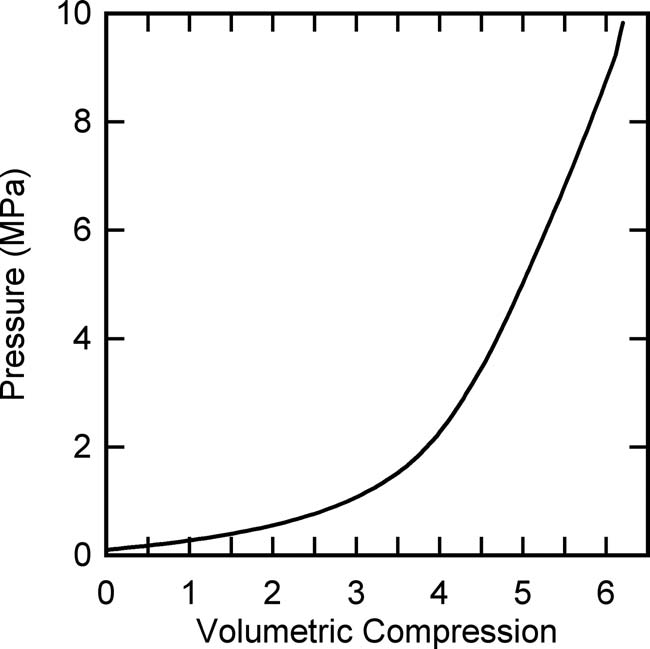
\includegraphics[width=3.0in]{figs/air_eos.png}                 
  \end{center}                                                                   
 \caption{Illustration of air pressure as a function of volumetric compression
 at ambient conditions.  (Taken from Fig.~2 of Taylor 2009.)}
 \label{fig:air_eos}
\end{figure}                                                                   




%====================
\section{Boundary Conditions}
%====================
\subsubsection{Energized Air}
A volume of energized air (elevated from ambient in both [internal] energy and
pressure was positioned 16~cm from the head.  This produces a blast wave
of 1,300~kPa (13~bars = 188.5~psi) propagating through ambient air.
The pressure wave is shown in Fig.~\ref{fig:blast_pressure}.  

\begin{figure}[htb]                                                            
  \begin{center}                                                                
  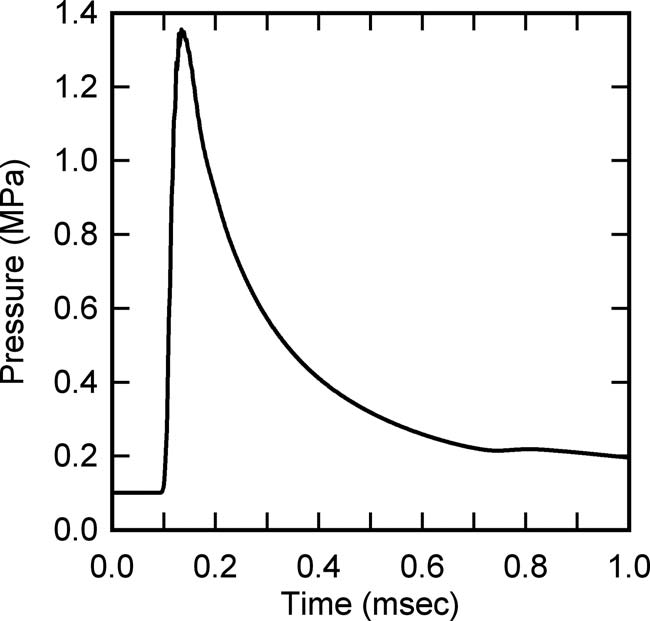
\includegraphics[width=3.15in]{figs/blast_pressure.png}
  \end{center}                                                                   
 \caption{Illustration of blast air pressure pulse as a function of 
 time (for a discrete? position in space, e.g., in front of the head?).
 (Taken from Fig.~3 of Taylor 2009.)}
 \label{fig:blast_pressure}
\end{figure}                                                                   





According Taylor,\footnote{Taylor PA, Ludwigsen JS, Ford CC. 
Investigation of blast-induced traumatic brain injury. 
Brain injury. 2014 Jun 1;28(7):879-95.} 
\begin{quotation}
Originally, blast conditions were selected consisting of 
1.35~MPa (13.5 bar) peak amplitude and a pulse width of 0.6~milliseconds,
which were within the marginal limits for threshold lung
damage, as defined by the corrected Bowen survivability curve for
blast injury [23] (see Figure 3).  These conditions were chosen for two
reasons.  First, they were similar to those predicted to occur at a 
location roughly 3~metres distant from a detonated explosive device
constructed from a 3~kg charge of Octol explosive.  
Second, they represented a limiting case for blast exposure predicted 
to be survivable by the Bowen lung damage criterion.  However, for this
blast condition, the results predicted that this strong of a blast
generated intracranial stress and energy levels that were too great to
be associated with mild traumatic brain injury (mTBI), the severity of
brain injury displayed by this clinical TBI subject group.
\end{quotation}


\begin{figure}[htb]                                                            
  \begin{center}                                                                
  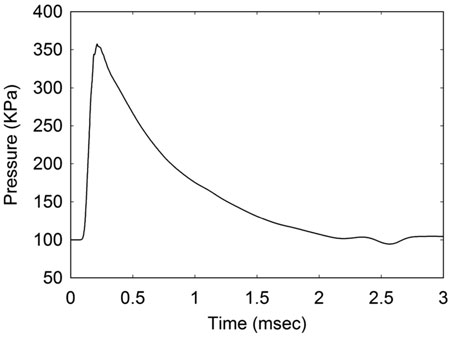
\includegraphics[width=0.8\textwidth]{figs/taylor_2014_fig_4.png}
  \end{center}                                                                   
 \caption{Illustration of blast air pressure pulse as a function of
 time (for a discrete? position in space, e.g., in front of the head?).
 (Taken from Fig.~4 Taylor 2014.)}
 \label{fig:taylor_2014_fig_4}
\end{figure}                                                                   


Taylor continued,\footnote{Taylor 2014 \opcit}
\begin{quotation}
As an alternative, blast conditions were selected that would be less
damaging to facial bone structure and more in line with conditions
leading to mTBI but still close to the limits for threshold lung damage.  
Furthermore, since this study was interested in conditions that a 
warfighter might experience during exposure to IED detonation, a blast 
history was selected that would result from a 2.3~kg charge of 
Composition-4 (C-4) located 2.3~metres from the head-neck model.  
This explosion produces an air blast of magnitude 360~KPa (3.6 bars)
with a pulse width of 2.0~milliseconds as it encounters the head-neck
model.  A profile of this blast is displayed in 
Figure~4 [Fig.~\ref{fig:taylor_2014_fig_4} herein].  
Both the 1.35~MPa and 360~KPa blast pulses are plotted in 
Figure~3 [Fig.~\ref{fig:taylor_2014_fig_3} herein], showing their
proximity to the Bowen curve for threshold lung damage and its 
correction~[23].
\end{quotation}

\begin{figure}[htb]                                                            
  \begin{center}                                                                
  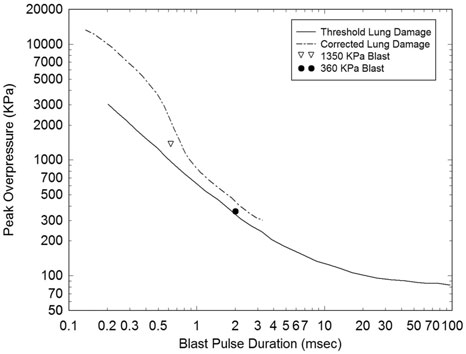
\includegraphics[width=0.8\textwidth]{figs/taylor_2014_fig_3.png}
  \end{center}                                                                   
 \caption{Threshold lung damage peak overpressure versus time pulse
 duration, with (overpressure, duration) data points shown at
 (1.35~MPa, 0.6~ms) and (360~kPa, 2.0~ms).
 (Taken from Fig.~3 Taylor 2014.)}
 \label{fig:taylor_2014_fig_3}
\end{figure}                                                                   

\clearpage
%====================
\section{CTH Implementation}
%====================
\subsection{Skull}


\begin{verbatim}
package 'Skull'
  iter 6
  material 4
  pressure 1.e6
  insert stl
    file = 'Brain_Axial_cut_skull-1.STL'
  endinsert
endpackage
\end{verbatim}

\begin{verbatim}
*Equation-of-State (EOS) Specification (Volumetric Response)

eos
*eosfile='home/pataylo/cth_6_6_2014/SkyBSrDam2/cth/data/EOS_data'

* ------------------
* Mie-Gruneisen Bone
* ------------------ 
  mat4 mgr user      g0=1.0      cs=1.9838e5     cv=1.0e10
       r0=1.210      s1=1.0
\end{verbatim}
From the CTH user manual, page 52:
\begin{itemize}
\item {\tt cs} = sound speed
\item {\tt cv} = specific heat
\item {\tt g0} = Gr{\"u}neisen parameter
\item {\tt r0} = initial density of Hugoniot\footnote{Also gives 
           default initial density if 
           material is not porous.  If the material is porous, parameter 
	   {\tt rp} specifies initial density and {\tt r0} is ambient density for 
	   nonporous solid.}
\item {\tt s1} = linear coefficient of the US-UP Hugoniot curve
\end{itemize}


\begin{verbatim}
* ---------------------------------
* Deviatoric Strength Specification
* ---------------------------------

*fvp='/home/pataylo/cth/cth_6_6_2014/SkyBSrDam2/cth/data/VP_data'

*Bone:
  matep 4   eppvm=user    yield=0.95e9    poisson=0.22    tmelt=1.0
            jfrac=user    jfpf0=-0.775e9  jfd1=0.100      jfd2=0.0
	    jfd3=0        jfd4=0          jfd5=0          jftm=1.e20

\end{verbatim}


\subsection{White Matter}

\subsection{Gray Matter}

\subsection{Cerebral Spinal Fluid (CSF)}

\subsection{Dry Air}



\clearpage
%====================
\section{ALEGRA Implementation}
%====================
Need to match material models in CTH to ALEGRA.

%====================
\section{Notes}
%====================
\begin{itemize}
\item From Taylor 2009, ``A typical blast simulation required 31 h using 64 
processors on the Sandia National Laboratories Thunderbird computer to 
integrate out to a time of 2~ms for a 16.72~$\times$~10$^6$ cell calculation.''
\end{itemize}



%====================
\section{Questions for Paul}
%====================
\begin{itemize}
\item Why keep the critical value of equivalent plastic strain inside the 
time interval, or at least confirm this ``critical value'' is time-independent.
\item Do we ever see fully damaged material $D=1$ in our sims?
\item If we have fully damaged material, do we have a loss of ellipticity 
for the strength equations?
\item What strain tensor is being described the equivalent plastic strain?
\item Is Mie-Gr\"uneisen equation of state restricted to the use of solids
only, or can it be applied to liquids and gases too?
\end{itemize}

%====================
\pagebreak
\appendix
\section{Details on Material Models}
%====================

\subsection{Mie-\Gru Equation of State}
The Mie-\Gru equation of state (MGEOS) is relationship between pressure $P$
and volume $V$ of a solid [ask Paul if just a solid, 
or applicable to liquid and gas too?] at a given temperature $T$.  
The work was originally published by Mie\footnote{Mie G. Zur kinetischen 
Theorie der einatomigen Körper. Annalen der Physik. 1903 Jan 1;316(8):657-97.}
in~1903 and then later in \Gru\footnote{\Gru E. 
Theorie des festen Zustandes einatomiger Elemente. 
Annalen der Physik. 1912 Jan 1;344(12):257-306.} in~1912.  

The development of the MGEOS starts from the \Gru model that states the
\Gru parameter $\Gamma$, a parameter that describes thermal pressure 
from a set of vibrating atoms, is related to pressure $P$ and internal
energy $U$ through
\be
\Gamma = V \left( \frac{dP}{dU} \right)_V.
\ee
Assume, next, that the \Gru parameter $\Gamma$ is independent of 
pressure $P$ and internal energy $U$.  Then the foregoing equation
can be rewritten as
\begin{align}
  dP = \frac{\Gamma}{V} \; dU, \\
  \int dP = \frac{\Gamma}{V} \int dU.  \\
\end{align}
Next, integrate the foregoing equation from 
$P_0$ and $U_0$, which exist at the $0$ 
reference state, 
usually assumed to be absolute freezing, $0^{\circ}$~Kelvin, 
Assume $P_0$ and $U_0$ are independent of of temperature $T$ and that
pressure $P$ and internal energy $U$ can be estimated from the 
Hugoniot equations.  This gives
\be
 P - P_0 = \frac{\Gamma}{V} \left(U - U_0 \right).
\ee

Next, consider the Hugoniot equations for conservation of mass, 
momentum, and energy.  
The Hugoniot equation for conservation of mass relates 
reference density $\rho_0$, density due to shock compression $\rho$,
shock velocity $v_s$, and particle velocity $v_p$, as
\be
 \rho_0 v_s = \rho \left( v_s - v_p \right).
\ee



%====================
\pagebreak
\section{Vector Algebra and Calculus Notes}
%====================
As defined by Gurtin,\footnote{Gurtin ME. An introduction to 
continuum mechanics. Academic press; 1982, Vol.~158, Jan 12.}
\begin{itemize}
\item \lin =  the set of all tensors
\item \linplus =  the set of all sensors $\vS$ with $\det \vS > 0$
\item \sym =  set of all symmetric tensors
\item \skw =  set of all skew tensors
\item \psym =  set of all positive definite, symmetric tensors
\item \orth =  set of all orthogonal tensors
\item \orthplus =  set of all rotations  
\end{itemize}



As defined by Curnier,\footnote{Curnier A. Computational methods 
in solid mechanics. Springer Science \& Business Media; 2012 Dec 6.}
for all second-order tensors $\vS \in$~\lin, 
the {\bf tracor} $\mathbb{T}$ and {\bf deviator} $\mathbb{D}$ 
are fourth-order tensors are defined as
\be
 \mathbb{T} \defe \frac{1}{3} \delta_{ij} \delta_{kl} \; 
 \veeihat \otimes
 \veejhat \otimes 
 \veekhat \otimes
 \veelhat 
\ee
such that 
\be
 \mathbb{T} \vddiv \vS = \vS_{\smvol} 
 \defe \frac{1}{3} \trace(\vS)\vid, 
\ee
and
\be
 \mathbb{D} \defe 
 \left(
 \frac{1}{2} \delta_{ik} \delta_{jl} +
 \frac{1}{2} \delta_{il} \delta_{jk} - 
 \frac{1}{3} \delta_{ij} \delta_{kl} \; 
 \right)
 \veeihat \otimes
 \veejhat \otimes 
 \veekhat \otimes
 \veelhat 
\ee
such that
\be
 \mathbb{D} \vddiv \vS = \vS_{\smdev}, 
 \defe \vS - \frac{1}{3} \trace(\vS)\vid.
\ee
Note, there are two other fourth-order tensors often used, 
the {\bf symmetrizer} $\mathbb{S}$ and the {\bf skewer} $\mathbb{W}$
defined, respectively, as 
\be
 \mathbb{S} \defe 
 \frac{1}{2}
 \left(
 \delta_{ik} \delta_{jl} +
 \delta_{il} \delta_{jk} 
 \right)
 \veeihat \otimes
 \veejhat \otimes 
 \veekhat \otimes
 \veelhat,
\ee
and
\be
 \mathbb{W} \defe 
 \frac{1}{2}
 \left(
 \delta_{ik} \delta_{jl} -
 \delta_{il} \delta_{jk} 
 \right)
 \veeihat \otimes
 \veejhat \otimes 
 \veekhat \otimes
 \veelhat.
\ee


\end{document}







